\section{Simulazioni modello di Ising 1D}

%-----------------------------------------%
%				Prima slide				  %
%	   Caratterizzazione del modello   	  %
%-----------------------------------------%
\begin{frame}
    \frametitle{Caratterizzazione}
    \framesubtitle{}

    \begin{columns}
        \begin{column}{0.33\textwidth}
            \begin{block}{Termalizzazione}

                \begin{itemize}[itemsep=0.5em, label=$\diamond$]
                    \item Maggiore T, minore $t_{term}$
                    \item $t_{term}^{max}\,\simeq\,600$ sweeps
                \end{itemize}

                \vspace{0.5cm}

                \centering
                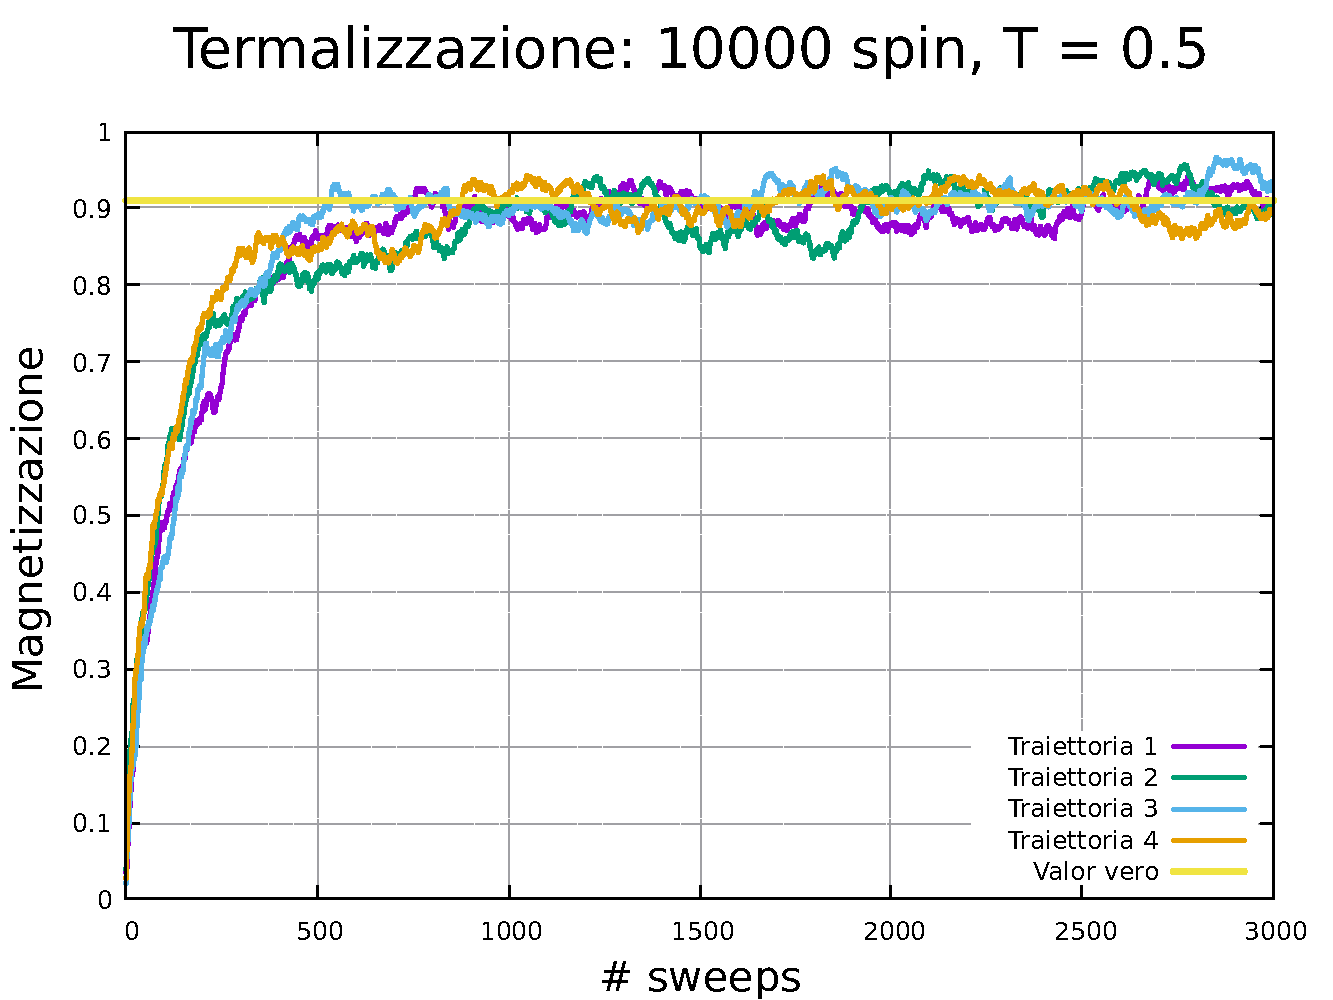
\includegraphics[width=\textwidth]{Immagini/simIsing1D/term_10000_1.5.pdf}
            
            \end{block}
        \end{column}
    
        \begin{column}{0.33\textwidth}
            \begin{block}{Auto-correlazione}

                \begin{itemize}[itemsep=0.5em, label=$\diamond$]
                    \item Maggiore T, minore $t_{c}$
                    \item $t_{c}^{max}\,\simeq\,500$ sweeps
                \end{itemize}

                \vspace{0.5cm}

                \centering
                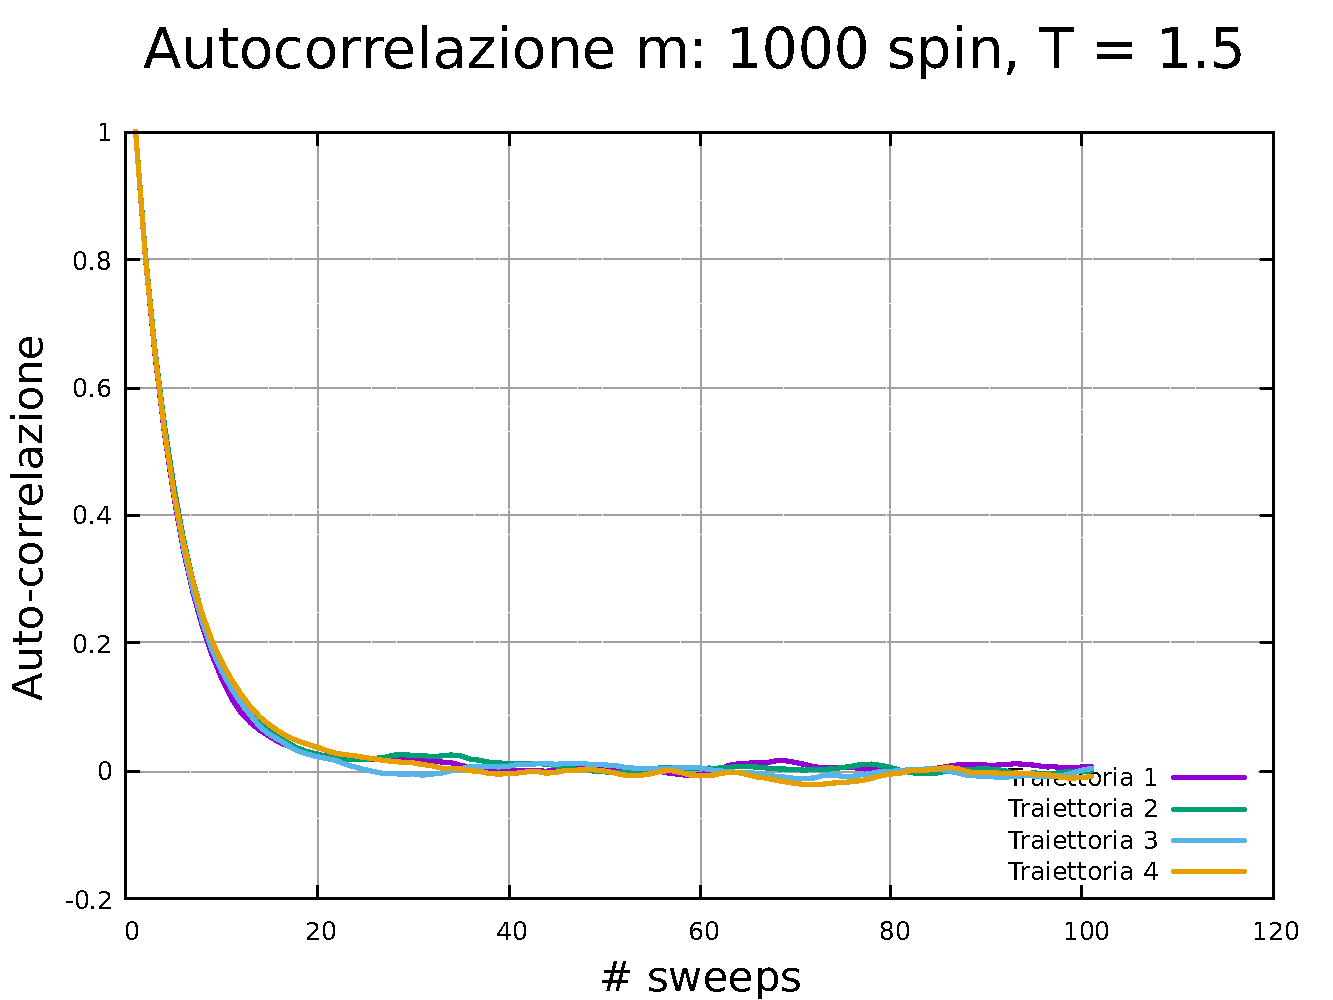
\includegraphics[width=\textwidth]{Immagini/simIsing1D/auto_1000_1.5.pdf}
            
            \end{block}
        \end{column}

        \begin{column}{0.33\textwidth}
            \begin{block}{Blocchi}
                \begin{itemize}[itemsep=0.5em, label=$\diamond$]
                    \item Maggiore T, minore $l_{blk}$
                    \item $l_{blk}^{max}\,\simeq\,1000$ sweeps
                \end{itemize}

                \vspace{0.5cm}

                \centering
                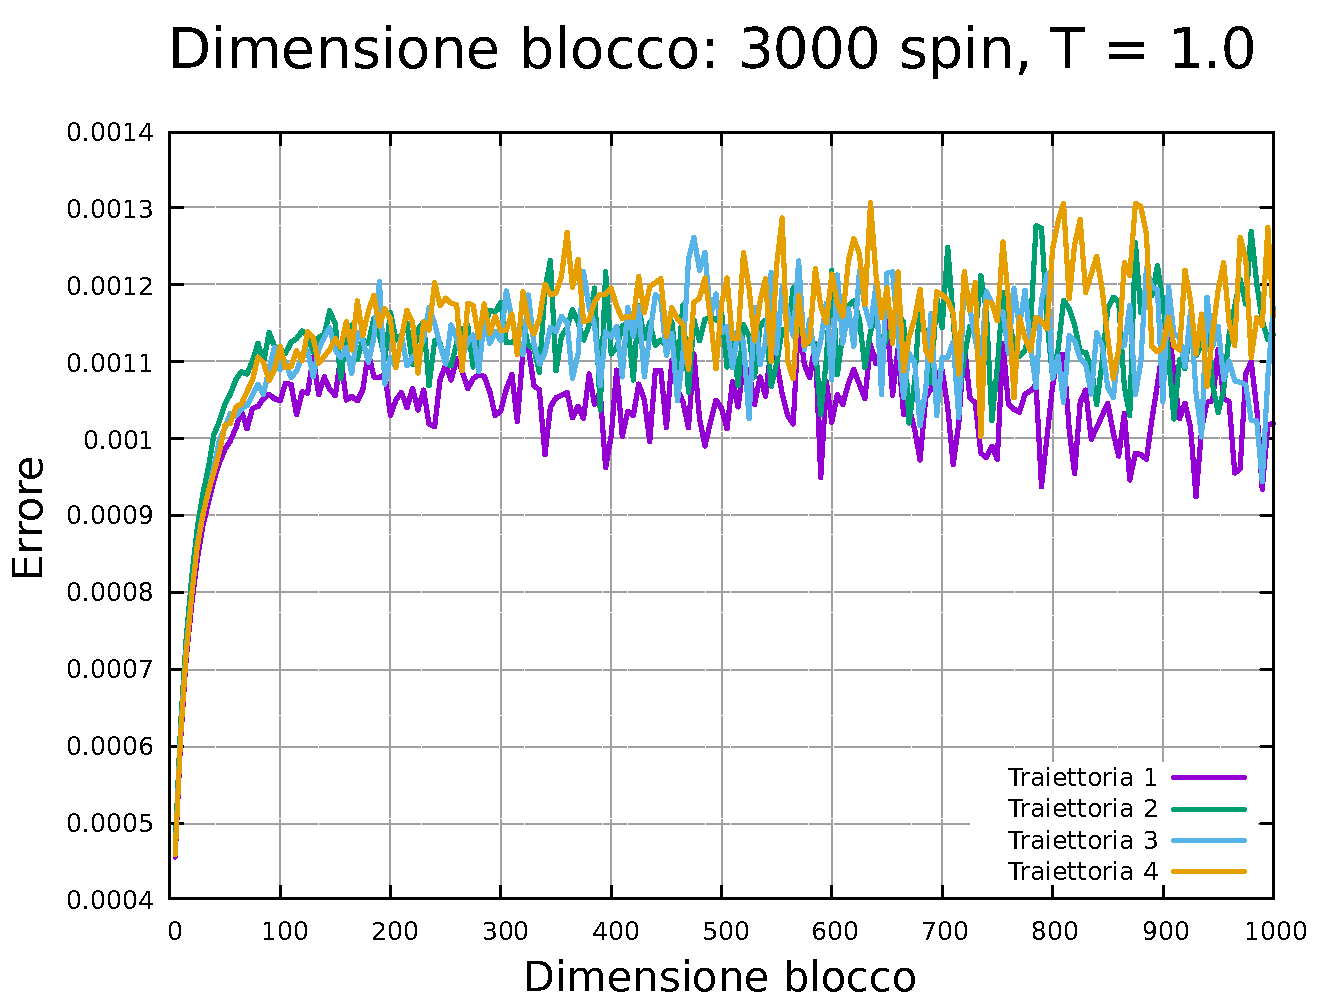
\includegraphics[width=\textwidth]{Immagini/simIsing1D/err_3000_1.0.pdf}
            \end{block}        
        \end{column}
    \end{columns}
\end{frame}



%-----------------------------------------%
%			  Seconda slide				  %
%	   Studio della magnetizzazione   	  %
%-----------------------------------------%
\begin{frame}
    \frametitle{Magnetizzazione}
    \framesubtitle{}

    \begin{columns}
        \begin{column}{0.5\textwidth}
            \begin{block}{$h\,=\,0.0$}

            \centering
            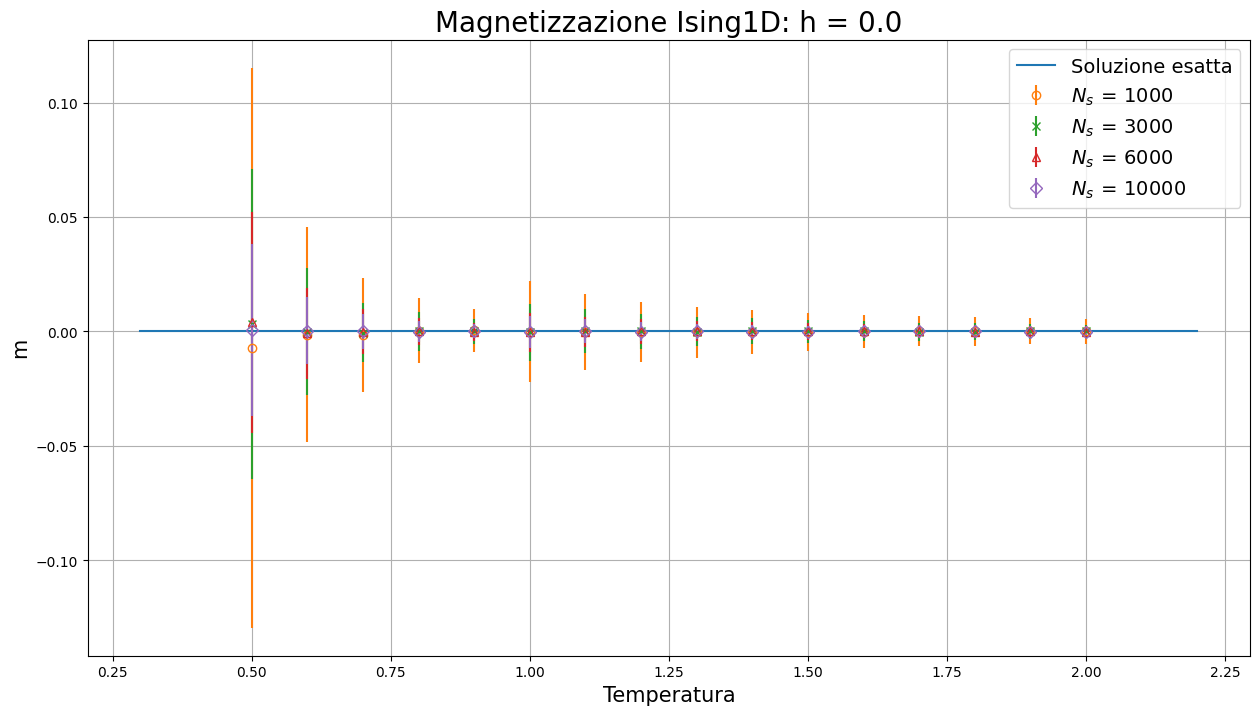
\includegraphics[width=\textwidth]{Immagini/simIsing1D/magn_h0.0.png}

            \vspace{0.5cm}
            \begin{itemize}[itemsep=0.5em, label=$\diamond$]
                \item $m\,=\,0$ per ogni $T \neq 0$
            \end{itemize}
            
            \end{block}
        \end{column}
    
        \begin{column}{0.5\textwidth}
            \begin{block}{$h\,=\,0.02$}

                \centering
                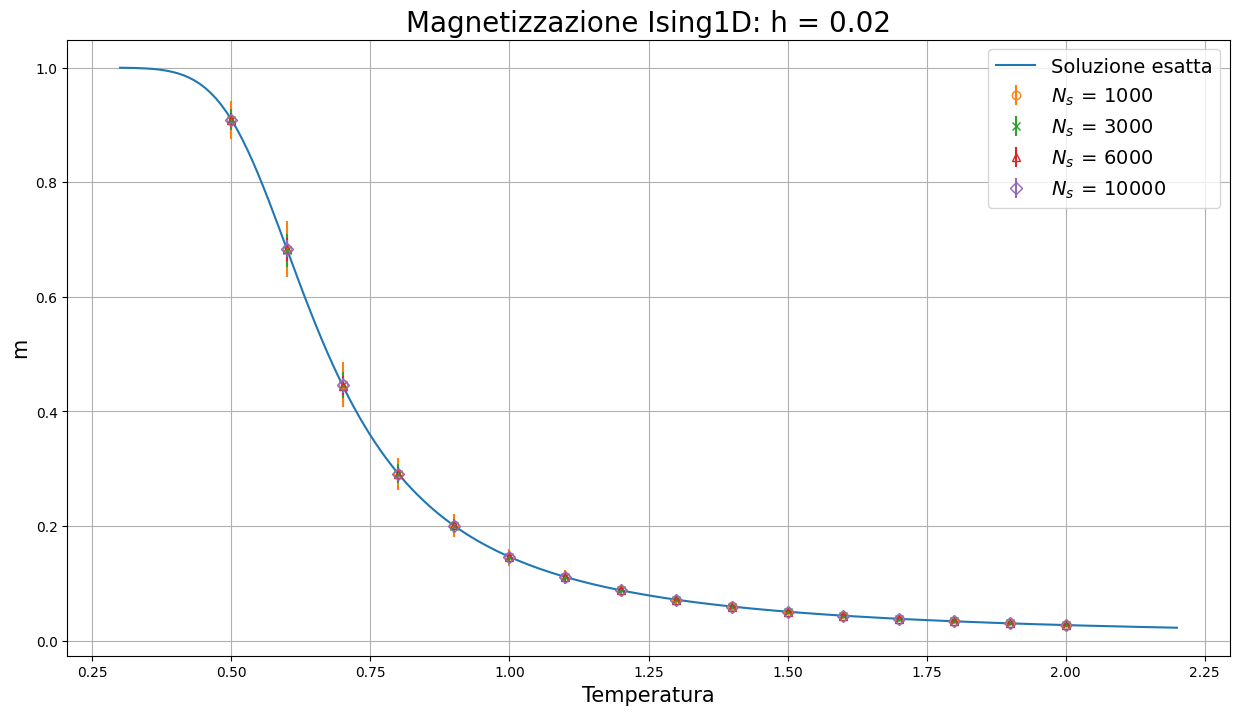
\includegraphics[width=\textwidth]{Immagini/simIsing1D/magn_h0.02.png}

                \vspace{0.5cm}
                \begin{itemize}[itemsep=0.5em, label=$\diamond$]
                    \item campo magnetico impone ordine
                \end{itemize}
            
            \end{block}
        \end{column}
    \end{columns}

\end{frame}



%-----------------------------------------%
%			  Terza slide				  %
%	   Studio dell'energia interna   	  %
%-----------------------------------------%
\begin{frame}
    \frametitle{Energia interna}
    \framesubtitle{}

    \begin{columns}
        \begin{column}{0.5\textwidth}
            \begin{block}{$h\,=\,0.0$}

            \centering
            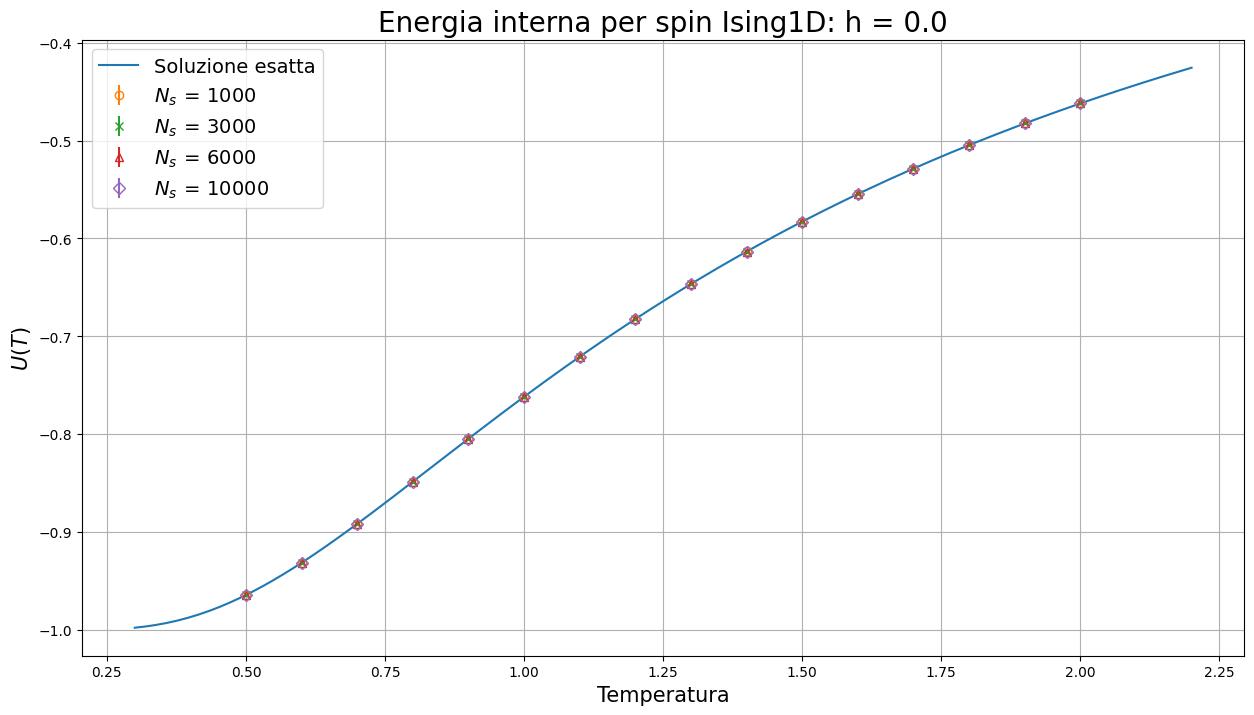
\includegraphics[width=\textwidth]{Immagini/simIsing1D/ene_h0.0.png}

            \vspace{0.5cm}
            \begin{itemize}[itemsep=0.5em, label=$\diamond$]
                \item per $T \to 0$ l'energia $U\left(T\right) \to -1$
            \end{itemize}
            
            \end{block}
        \end{column}
    
        \begin{column}{0.5\textwidth}
            \begin{block}{$h\,=\,0.02$}

                \centering
                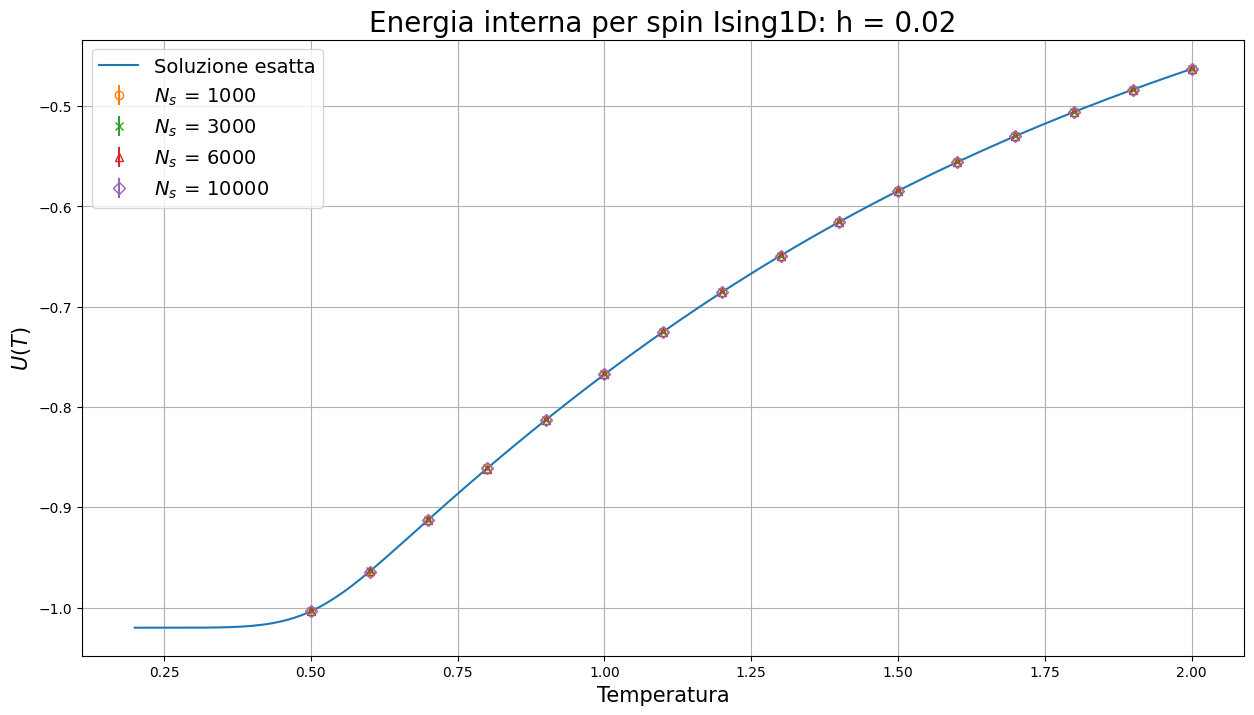
\includegraphics[width=\textwidth]{Immagini/simIsing1D/ene_h0.02.png}

                \vspace{0.5cm}
                \begin{itemize}[itemsep=0.5em, label=$\diamond$]
                    \item per $T \to 0$ l'energia $U\left(T\right) \to -1.02$
                \end{itemize}
            
            \end{block}
        \end{column}
    \end{columns}

\end{frame}



%-----------------------------------------%
%		   	  Quarta slide				  %
%	    Studio della suscettività   	  %
%-----------------------------------------%
\begin{frame}
    \frametitle{Suscettività magnetica}
    \framesubtitle{}

    \begin{columns}
        \begin{column}{0.5\textwidth}
            \begin{block}{$h\,=\,0.0$}

            \centering
            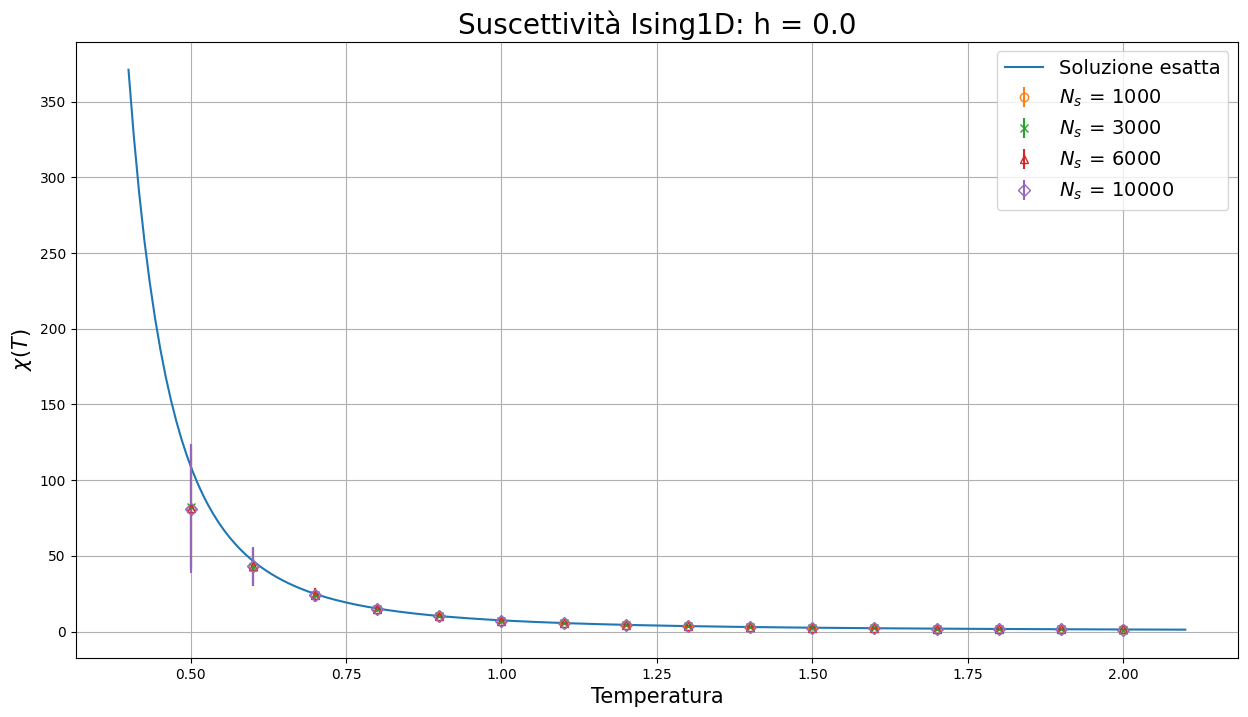
\includegraphics[width=\textwidth]{Immagini/simIsing1D/chi_h0.0.png}

            \vspace{0.5cm}
            \begin{itemize}[itemsep=0.5em, label=$\diamond$]
                \item aumento per $T \to 0$ perchè $T_c\,=\,0$
            \end{itemize}
            
            \end{block}
        \end{column}
    
        \begin{column}{0.5\textwidth}
            \begin{block}{$h\,=\,0.02$}

                \centering
                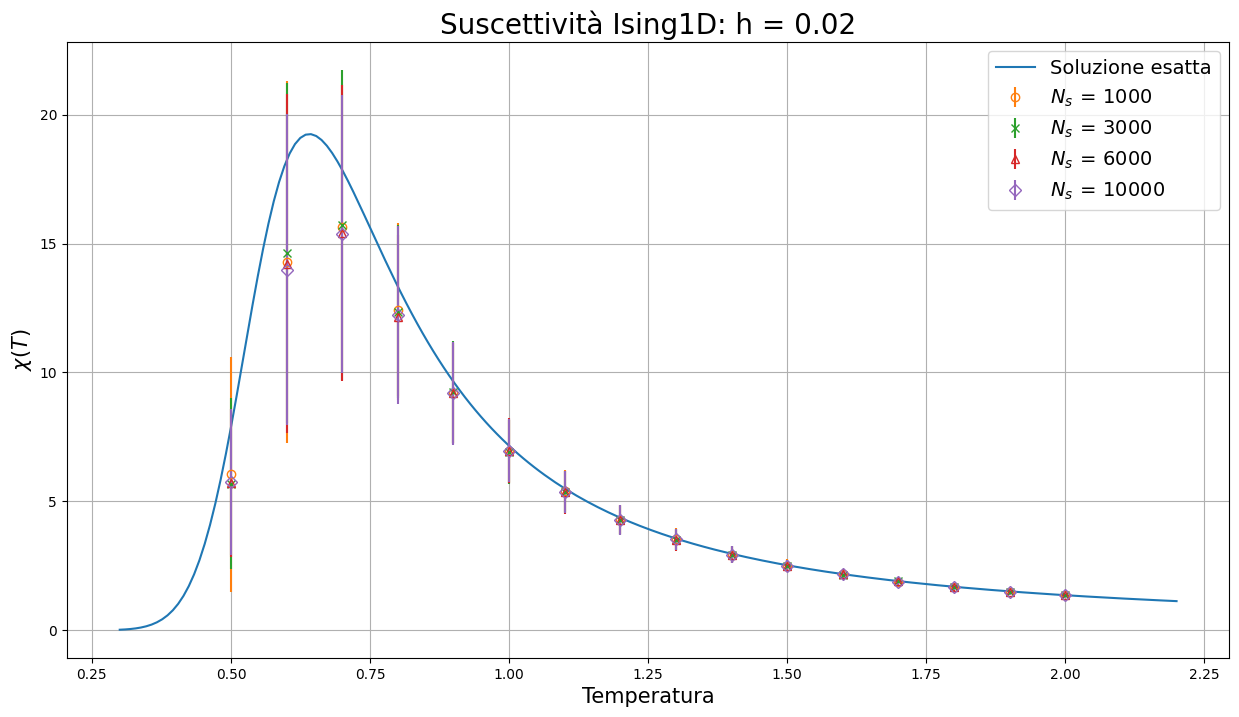
\includegraphics[width=\textwidth]{Immagini/simIsing1D/chi_h0.02.png}

                \vspace{0.5cm}
                \begin{itemize}[itemsep=0.5em, label=$\diamond$]
                    \item picco a $T \neq 0$ dovuto ad $h$
                \end{itemize}
            
            \end{block}
        \end{column}
    \end{columns}

\end{frame}



%-----------------------------------------%
%		   	  Quinta slide				  %
%	    Studio del calore specifico   	  %
%-----------------------------------------%
\begin{frame}
    \frametitle{Calore specifico}
    \framesubtitle{}

    \begin{columns}
        \begin{column}{0.5\textwidth}
            \begin{block}{$h\,=\,0.0$}

            \centering
            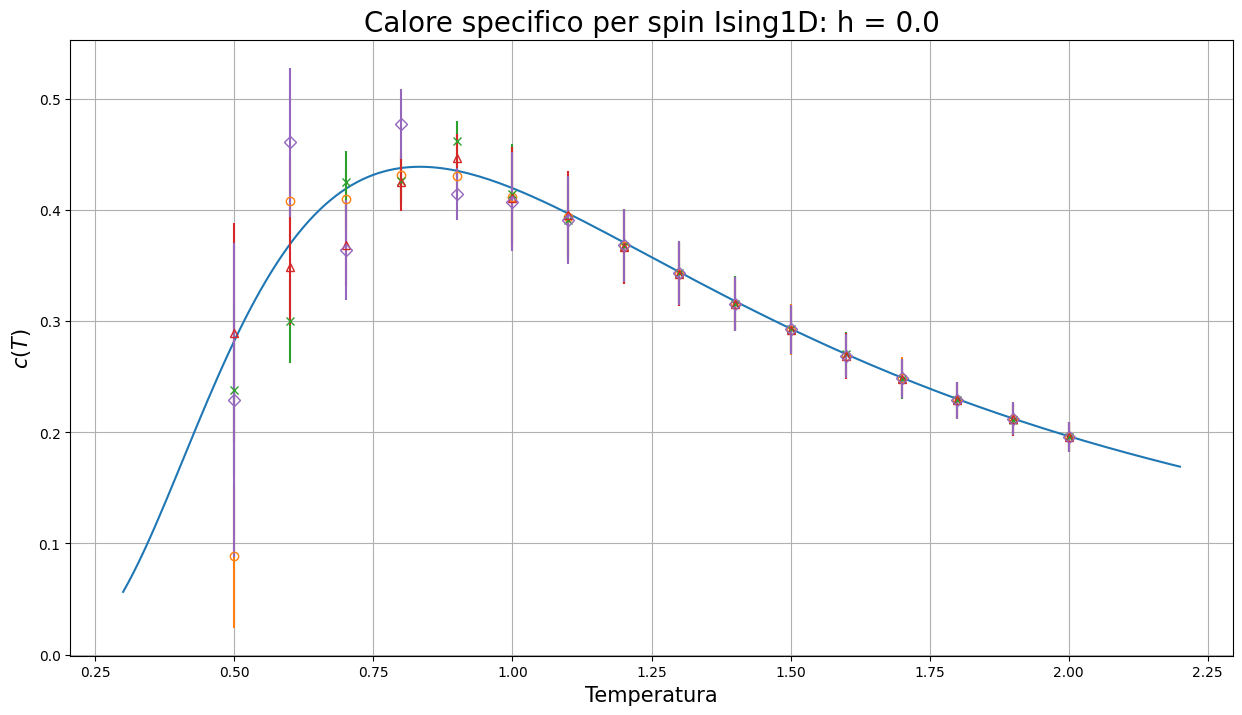
\includegraphics[width=\textwidth]{Immagini/simIsing1D/cp_h0.0.png}

            \vspace{0.5cm}
            \begin{itemize}[itemsep=0.5em, label=$\diamond$]
                \item difficoltà a studiare il picco
            \end{itemize}
            
            \end{block}
        \end{column}
    
        \begin{column}{0.5\textwidth}
            \begin{block}{$h\,=\,0.02$}

                \centering
                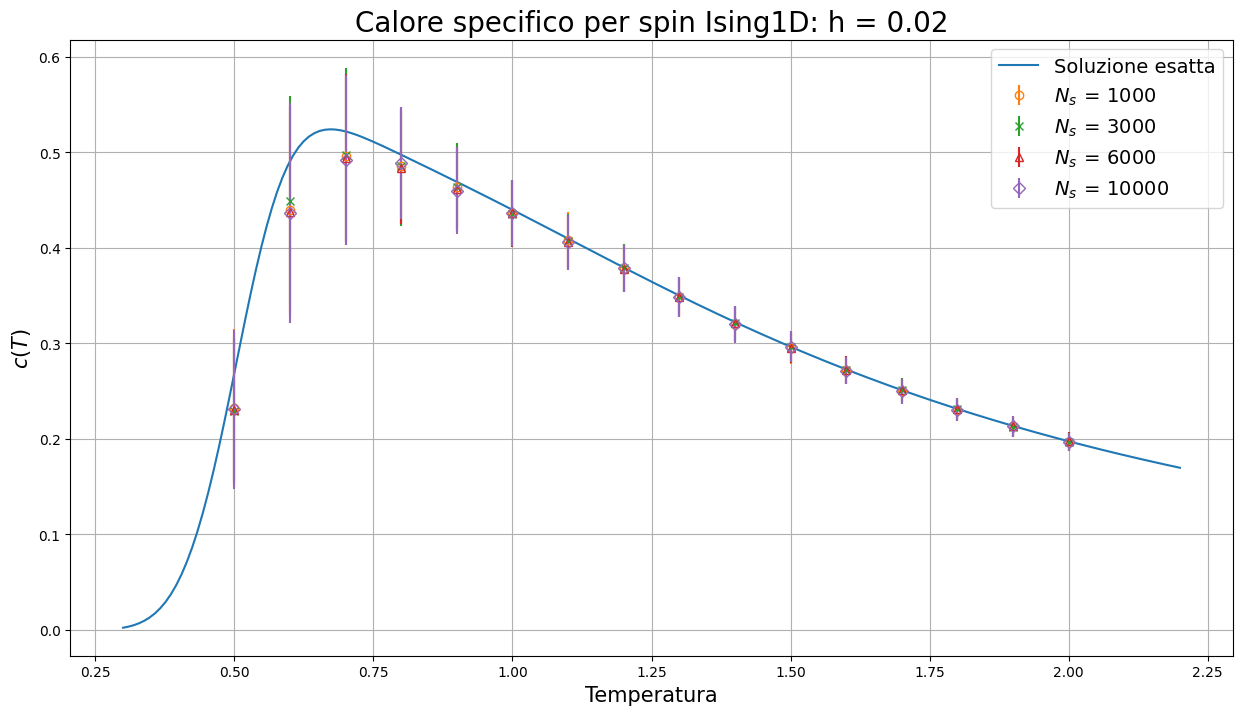
\includegraphics[width=\textwidth]{Immagini/simIsing1D/cp_h0.02.png}

                \vspace{0.5cm}
                \begin{itemize}[itemsep=0.5em, label=$\diamond$]
                    \item campo magnetico semplifica lo studio
                \end{itemize}
            
            \end{block}
        \end{column}
    \end{columns}

\end{frame}